
\section{Hyperbolic Functions Revisited}\label{sec:inv hyperbolic}\label{sec:hyperbolic revisited}

In Section \ref{sec:hyperbolic functions} we introduced the hyperbolic functions.  From Definition \ref{def:hyperbolic_functions} we recall their respective definitions. 

\begin{enumerate}
\item		$\ds \cosh x = \frac{e^x+e^{-x}}2$
\item		$\ds \sinh x = \frac{e^x-e^{-x}}2$
\item		$\ds \tanh x = \frac{\sinh x}{\cosh x}$
\item		$\ds \sech x = \frac{1}{\cosh x}$
\item		$\ds \csch x = \frac{1}{\sinh x}$
\item		$\ds \coth x = \frac{\cosh x}{\sinh x}$
\end{enumerate}


\begin{example}{Exploring properties of hyperbolic functions}{ex_hf1}
{
Use the definitions of the hyperbolic functions to rewrite the following expressions.
\begin{enumerate}
\item		$\frac{d}{dx}\big(\cosh x\big)$
\item		$\frac{d}{dx}\big(\sinh x\big)$
\item		$\frac{d}{dx}\big(\tanh x\big)$
\end{enumerate}
}
\end{example}


\begin{solution}
{\begin{enumerate}
\item  \hfill$\begin{aligned}[t]
	\frac{d}{dx}\big(\cosh x\big) &= \frac{d}{dx}\left(\frac{e^x+e^{-x}}2\right) \\
					&= \frac{e^x-e^{-x}}2\\
					&= \sinh x.
	\end{aligned}\hfill$

So $\frac{d}{dx}\big(\cosh x\big) = \sinh x.$
	
\item  \hfill$\begin{aligned}[t]
	\frac{d}{dx}\big(\sinh x\big) &= \frac{d}{dx}\left(\frac{e^x-e^{-x}}2\right) \\
					&= \frac{e^x+e^{-x}}2\\
					&= \cosh x.
	\end{aligned}\hfill$

So $\frac{d}{dx}\big(\sinh x\big) = \cosh x.$
	
\item  \hfill$\begin{aligned}[t]
	\frac{d}{dx}\big(\tanh x\big) &= \frac{d}{dx}\left(\frac{\sinh x}{\cosh x}\right) \\
					&= \frac{\cosh x \cosh x - \sinh x \sinh x}{\cosh^2 x}\\
					&= \frac{1}{\cosh^2 x}\\
					&= \sech^2 x.
	\end{aligned}\hfill$

So $\frac{d}{dx}\big(\tanh x\big) = \sech^2 x.$	
\end{enumerate}
\vskip-\baselineskip
}
\end{solution}



The following Key Idea summarizes many of the important identities relating to hyperbolic functions. Each can be verified by referring back to Definition \ref{def:hyperbolic_functions}.


\begin{formulabox}[Useful Hyperbolic Function Properties]
\label{idea:hyperbolic_identities}
\footnotesize{\begin{minipage}[t]{.33\textwidth}
\textbf{Basic Identities}\par
\begin{enumerate}
\item $\cosh^2x-\sinh^2x=1$%
\index{hyperbolic function!identities}\index{hyperbolic function!derivatives}\index{hyperbolic function!integrals}\index{derivative!hyperbolic funct.}\index{integration!hyperbolic funct.}%
\item	$\tanh^2x+\sech^2x=1$
\item	$\coth^2x-\csch^2x = 1$
\item	$\cosh 2x=\cosh^2x+\sinh^2x$
\item	$\sinh 2x = 2\sinh x\cosh x$
\item	$\ds\cosh^2x = \frac{\cosh 2x+1}{2}$
\item $\ds \sinh^2x=\frac{\cosh 2x-1}{2}$
\end{enumerate}
\end{minipage}
\begin{minipage}[t]{.33\textwidth}
\textbf{Derivatives}
\begin{enumerate}
\item $\frac{d}{dx}\big(\cosh x\big) = \sinh x$
\item $\frac{d}{dx}\big(\sinh x\big) = \cosh x$
\item $\frac{d}{dx}\big(\tanh x\big) = \sech^2 x$
\item $\frac{d}{dx}\big(\sech x\big) = -\sech x\tanh x$
\item $\frac{d}{dx}\big(\csch x\big) = -\csch x\coth x$
\item $\frac{d}{dx}\big(\coth x\big) = -\csch^2x$
\end{enumerate}
\end{minipage}
\begin{minipage}[t]{.33\textwidth}
\textbf{Integrals}
\begin{enumerate}
\item $\ds\int \cosh x\ dx = \sinh x+C$
\item $\ds\int \sinh x\ dx = \cosh x+C$
\item $\ds\int \tanh x\ dx = \ln(\cosh x) +C$
\item $\ds\int \coth x\ dx = \ln|\sinh x\,|+C$
\end{enumerate}
\end{minipage}
}
\end{formulabox}




Next, we practice using these properties.\\

\begin{example}{Derivatives and integrals of hyperbolic functions}{ex_hf2}
{
Evaluate the following derivatives and integrals.

\begin{minipage}[t]{.5\linewidth}
\begin{enumerate}
\item		$\ds\frac{d}{dx}\big(\cosh 2x\big)$
\item		$\ds\int \sech^2(7t-3)\ dt$
\end{enumerate}
\end{minipage}
\begin{minipage}[t]{.5\linewidth}
\begin{enumerate}\addtocounter{enumi}{2}
\item		$\ds \int_0^{\ln 2} \cosh x\ dx$
\end{enumerate}
\end{minipage}
}
\end{example}


\begin{solution}
{\begin{enumerate}
\item		Using the Chain Rule directly, we have $\frac{d}{dx} \big(\cosh 2x\big) = 2\sinh 2x$.

Just to demonstrate that it works, let's also use the Basic Identity found in Key Idea \ref{idea:hyperbolic_identities}: $\cosh 2x = \cosh^2x+\sinh^2x$.
\begin{align*}\frac{d}{dx}\big(\cosh 2x\big) = \frac{d}{dx}\big(\cosh^2x+\sinh^2x\big) &= 2\cosh x\sinh x+ 2\sinh x\cosh x\\ &= 4\cosh x\sinh x.
\end{align*}
Using another Basic Identity, we can see that $4\cosh x\sinh x = 2\sinh 2x$. We get the same answer either way.

\item	  We employ substitution, with $u = 7t-3$ and $du = 7dt$ to get:
$$ \int \sech^2 (7t-3)\ dt =\int \frac{1}{7}\sech^2 (u)\ du= \frac17\tanh (u) + C = \frac17\tanh (7t-3) + C.$$

\item		$$\int_0^{\ln 2} \cosh x\ dx = \sinh x\Big|_0^{\ln 2} = \sinh (\ln 2) - \sinh 0 = \sinh(\ln 2).$$
We can simplify this last expression as $\sinh x$ is based on exponentials:
$$\sinh(\ln 2) = \frac{e^{\ln 2}-e^{-\ln 2}}2 = \frac{2-1/2}{2} = \frac34.$$
\end{enumerate}
\vskip-1.5\baselineskip
}
\end{solution}





\noindent\textbf{\large Inverse Hyperbolic Functions}\\

Just as the inverse trigonometric functions are useful in certain integrations, the inverse hyperbolic functions are useful with others. Figure \ref{fig:hfinverse2} shows the restrictions on the domains to make each function one-to-one and the resulting domains and ranges of their inverse functions. Their graphs are shown in Figure \ref{fig:hfinverse1}.\index{hyperbolic function!inverse}

Because the hyperbolic functions are defined in terms of exponential functions, their inverses can be expressed in terms of logarithms as shown in Definition \ref{def:idea:hyperbolic_log}. It is often more convenient to refer to $\sinh^{-1}x$ than to $\ln\big(x+\sqrt{x^2+1}\big)$, especially when one is working on theory and does not need to compute actual values. On the other hand, when computations are needed, technology is often helpful but many hand-held calculators lack a \textit{convenient} $\sinh^{-1}x$ button. (Often it can be accessed under a menu system, but not conveniently.) In such a situation, the logarithmic representation is useful. The reader is not encouraged to memorize these, but rather know they exist and know how to use them when needed.

%\clearpage


\mtable{.7}{Graphs of $\cosh x$, $\sinh x$ and their inverses.}{fig:hfinverse3}{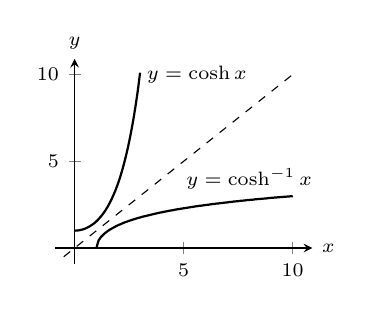
\begin{tikzpicture}
\begin{axis}[width=.4\textwidth,%
tick label style={font=\scriptsize},axis y line=middle,axis x line=middle,name=myplot,axis on top,%
			%x=.37\marginparwidth,
			%y=.37\marginparwidth,
%			xtick=\empty,% 
%			extra x ticks={.5,3},
%			extra x tick labels={$a$,$b$},
%			ytick={-.002,.002,.004},
%			yticklabels={$-0.002$,$0.002$,$0.004$},
			%minor y tick num=1,
%			extra y ticks={0.001},%
%			minor x tick num=4,
			ymin=-.9,ymax=10.9,%
			xmin=-.9,xmax=10.9,%
			scaled ticks=false
]

\addplot [{\colorone},thick,smooth] coordinates {(0,1.)(0.1,1.01) (0.2,1.02) (0.3,1.05) (0.4,1.08) (0.5,1.13) (0.6,1.19)(0.7,1.26) (0.8,1.34) (0.9,1.43) (1.,1.54) (1.1,1.67) (1.2,1.81) (1.3,1.97) (1.4,2.15) (1.5,2.35) (1.6,2.58) (1.7,2.83) (1.8,3.11)(1.9,3.42) (2.,3.76) (2.1,4.14) (2.2,4.57) (2.3,5.04) (2.4,5.56)
(2.5,6.13) (2.6,6.77) (2.7,7.47) (2.8,8.25) (2.9,9.11) (3.,10.1)};

\draw (axis cs:8,4) node {\scriptsize $y=\cosh^{-1} x$};
\draw (axis cs:5.6,10) node {\scriptsize $y=\cosh x$};

\addplot [{\colortwo},smooth,thick] coordinates {(1.,0)(1.1,0.444)(1.2,0.622)(1.3,0.756)(1.4,0.867)(1.5,0.962)(1.6,1.05)(1.7,1.12)(1.8,1.19)(1.9,1.26)(2.,1.32)(2.1,1.37)(2.2,1.43)(2.3,1.48)(2.4,1.52)(2.5,1.57)(2.6,1.61)(2.7,1.65)(2.8,1.69)(2.9,1.73)(3.,1.76)(3.1,1.8)(3.2,1.83)(3.3,1.86)(3.4,1.89)(3.5,1.92)(3.6,1.95)(3.7,1.98)(3.8,2.01)(3.9,2.04)(4.,2.06)(4.1,2.09)(4.2,2.11)(4.3,2.14)(4.4,2.16)(4.5,2.18)(4.6,2.21)(4.7,2.23)(4.8,2.25)(4.9,2.27)(5.,2.29)(5.1,2.31)(5.2,2.33)(5.3,2.35)(5.4,2.37)(5.5,2.39)(5.6,2.41)(5.7,2.43)(5.8,2.44)(5.9,2.46)(6.,2.48)(6.1,2.49)(6.2,2.51)(6.3,2.53)(6.4,2.54)(6.5,2.56)(6.6,2.57)(6.7,2.59)(6.8,2.6)(6.9,2.62)(7.,2.63)(7.1,2.65)(7.2,2.66)(7.3,2.68)(7.4,2.69)(7.5,2.7)(7.6,2.72)(7.7,2.73)(7.8,2.74)(7.9,2.76)(8.,2.77)(8.1,2.78)(8.2,2.79)(8.3,2.81)(8.4,2.82)(8.5,2.83)(8.6,2.84)(8.7,2.85)(8.8,2.86)(8.9,2.88)(9.,2.89)(9.1,2.9)(9.2,2.91)(9.3,2.92)(9.4,2.93)(9.5,2.94)(9.6,2.95)(9.7,2.96)(9.8,2.97)(9.9,2.98)(10.,2.99)};

\addplot [dashed,domain=-.5:10] {x};


%\draw (axis cs:2.4,-0.002) node {\scriptsize $f(x)$};
\end{axis}

\node [right] at (myplot.right of origin) {\scriptsize $x$};
\node [above] at (myplot.above origin) {\scriptsize $y$};
\end{tikzpicture} \hspace*{10pt}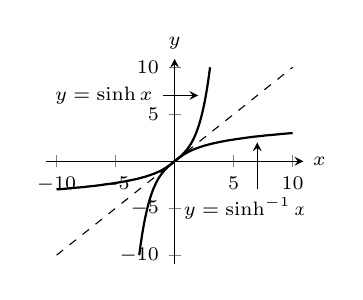
\begin{tikzpicture}
\begin{axis}[width=.4\textwidth,%
tick label style={font=\scriptsize},axis y line=middle,axis x line=middle,name=myplot,axis on top,%
			%x=.37\marginparwidth,
			%y=.37\marginparwidth,
%			xtick=\empty,% 
%			extra x ticks={.5,3},
%			extra x tick labels={$a$,$b$},
%			ytick={-.002,.002,.004},
%			yticklabels={$-0.002$,$0.002$,$0.004$},
			%minor y tick num=1,
%			extra y ticks={0.001},%
%			minor x tick num=4,
			ymin=-10.9,ymax=10.9,%
			xmin=-10.9,xmax=10.9,%
			scaled ticks=false
]

\addplot [{\colorone},thick,smooth] coordinates {(-3.,-10.) (-2.9,-9.06) (-2.8,-8.19) (-2.7,-7.41) (-2.6,-6.69)(-2.5,-6.05) (-2.4,-5.47) (-2.3,-4.94) (-2.2,-4.46) (-2.1,-4.02)(-2.,-3.63) (-1.9,-3.27) (-1.8,-2.94) (-1.7,-2.65) (-1.6,-2.38)(-1.5,-2.13) (-1.4,-1.9) (-1.3,-1.7) (-1.2,-1.51) (-1.1,-1.34)(-1.,-1.18) (-0.9,-1.03) (-0.8,-0.888) (-0.7,-0.759) (-0.6,-0.637)(-0.5,-0.521) (-0.4,-0.411) (-0.3,-0.305) (-0.2,-0.201) (-0.1,-0.1)(0,0) (0.1,0.1) (0.2,0.201) (0.3,0.305) (0.4,0.411) (0.5,0.521)(0.6,0.637) (0.7,0.759) (0.8,0.888) (0.9,1.03) (1.,1.18) (1.1,1.34)(1.2,1.51) (1.3,1.7) (1.4,1.9) (1.5,2.13) (1.6,2.38) (1.7,2.65)(1.8,2.94) (1.9,3.27) (2.,3.63) (2.1,4.02) (2.2,4.46) (2.3,4.94)(2.4,5.47) (2.5,6.05) (2.6,6.69) (2.7,7.41) (2.8,8.19) (2.9,9.06)(3.,10.) };

\draw (axis cs:-6,7) node {\scriptsize $y=\sinh x$};
\draw (axis cs:6,-5) node {\scriptsize $y=\sinh^{-1} x$};
\draw[->,>=stealth] (axis cs:-1,7) -- (axis cs:2,7);
\draw[->,>=stealth] (axis cs:7,-3) -- (axis cs:7,2);

\addplot [{\colortwo},smooth,thick] coordinates {(-10.,-3.)(-9.6,-2.96)(-9.2,-2.92)(-8.8,-2.87)(-8.4,-2.82)(-8.,-2.78)(-7.6,-2.73)(-7.2,-2.67)(-6.8,-2.62)(-6.4,-2.56)(-6.,-2.49)(-5.6,-2.42)(-5.2,-2.35)(-4.8,-2.27)(-4.4,-2.19)(-4.,-2.09)(-3.6,-1.99)(-3.2,-1.88)(-2.8,-1.75)(-2.4,-1.61)(-2.,-1.44)(-1.6,-1.25)(-1.2,-1.02)(-0.8,-0.733)(-0.4,-0.39)(0,0)(0.4,0.39)(0.8,0.733)(1.2,1.02)(1.6,1.25)(2.,1.44)(2.4,1.61)(2.8,1.75)(3.2,1.88)(3.6,1.99)(4.,2.09)(4.4,2.19)(4.8,2.27)(5.2,2.35)(5.6,2.42)(6.,2.49)(6.4,2.56)(6.8,2.62)(7.2,2.67)(7.6,2.73)(8.,2.78)(8.4,2.82)(8.8,2.87)(9.2,2.92)(9.6,2.96)(10.,3.)};

\addplot [dashed,domain=-10:10] {x};


%\draw (axis cs:2.4,-0.002) node {\scriptsize $f(x)$};
\end{axis}

\node [right] at (myplot.right of origin) {\scriptsize $x$};
\node [above] at (myplot.above origin) {\scriptsize $y$};
\end{tikzpicture}}

\mtable{.3}{Graphs of $\tanh^{-1} x$, $\coth^{-1} x$, $\sech^{-1} x$ and $\csch^{-1} x$.}{fig:hfinverse4}{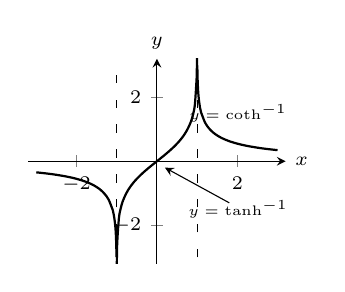
\begin{tikzpicture}
\begin{axis}[width=.4\textwidth,%
tick label style={font=\scriptsize},axis y line=middle,axis x line=middle,name=myplot,axis on top,%
			%x=.37\marginparwidth,
			%y=.37\marginparwidth,
			xtick={-2,2},%
%			xticklabels={$-1\qquad $,$\quad 1$}, 
%			extra x ticks={.5,3},
%			extra x tick labels={$a$,$b$},
			ytick={-2,2},
%			yticklabels={$-0.002$,$0.002$,$0.004$},
			%minor y tick num=1,
%			extra y ticks={0.001},%
%			minor x tick num=4,
			ymin=-3.2,ymax=3.2,%
			xmin=-3.2,xmax=3.2,%
			scaled ticks=false
]

%\addplot [{\colorone},thick,smooth] coordinates {(-3.,-0.995)(-2.9,-0.994)(-2.8,-0.993)(-2.7,-0.991)(-2.6,-0.989)(-2.5,-0.987)(-2.4,-0.984)(-2.3,-0.98)(-2.2,-0.976)(-2.1,-0.97)(-2.,-0.964)(-1.9,-0.956)(-1.8,-0.947)(-1.7,-0.935)(-1.6,-0.922)(-1.5,-0.905)(-1.4,-0.885)(-1.3,-0.862)(-1.2,-0.834)(-1.1,-0.8)(-1.,-0.762)(-0.9,-0.716)(-0.8,-0.664)(-0.7,-0.604)(-0.6,-0.537)(-0.5,-0.462)(-0.4,-0.38)(-0.3,-0.291)(-0.2,-0.197)(-0.1,-0.0997)(0,0)(0.1,0.0997)(0.2,0.197)(0.3,0.291)(0.4,0.38)(0.5,0.462)(0.6,0.537)(0.7,0.604)(0.8,0.664)(0.9,0.716)(1.,0.762)(1.1,0.8)(1.2,0.834)(1.3,0.862)(1.4,0.885)(1.5,0.905)(1.6,0.922)(1.7,0.935)(1.8,0.947)(1.9,0.956)(2.,0.964)(2.1,0.97)(2.2,0.976)(2.3,0.98)(2.4,0.984)(2.5,0.987)(2.6,0.989)(2.7,0.991)(2.8,0.993)(2.9,0.994)(3.,0.995)};

\addplot [{\colortwo},thick,smooth] coordinates {(1.005,2.997)(1.01,2.65)(1.02,2.31)(1.03,2.11)(1.04,1.97)(1.05,1.86)(1.06,1.77)(1.07,1.69)(1.08,1.63)(1.09,1.57)(1.1,1.52)(1.2,1.2)(1.3,1.02)(1.4,0.896)(1.5,0.805)(1.6,0.733)(1.7,0.675)(1.8,0.626)(1.9,0.585)(2.,0.549)(2.1,0.518)(2.2,0.49)(2.3,0.466)(2.4,0.444)(2.5,0.424)(2.6,0.405)(2.7,0.389)(2.8,0.374)(2.9,0.36)(3.,0.347)};

\addplot [{\colortwo},thick,smooth] coordinates {(-3.,-0.347)(-2.9,-0.36)(-2.8,-0.374)(-2.7,-0.389)(-2.6,-0.405)(-2.5,-0.424)(-2.4,-0.444)(-2.3,-0.466)(-2.2,-0.49)(-2.1,-0.518)(-2.,-0.549)(-1.9,-0.585)(-1.8,-0.626)(-1.7,-0.675)(-1.6,-0.733)(-1.5,-0.805)(-1.4,-0.896)(-1.3,-1.02)(-1.2,-1.2)(-1.1,-1.52)(-1.09,-1.57)(-1.08,-1.63)(-1.07,-1.69)(-1.06,-1.77)(-1.05,-1.86)(-1.04,-1.97)(-1.03,-2.11)(-1.02,-2.31)(-1.01,-2.65)(-1.005,-2.997)};

\draw (axis cs:2.2,1.5) node {\tiny $y=\coth^{-1} x$};
\draw (axis cs:2.2,-1.5) node {\tiny $y=\tanh^{-1} x$};
\draw [->,>=stealth] (axis cs:1.8,-1.3) -- (axis cs:.2,-.2);
%\draw [->,>=stealth] (axis cs:-.1,2.5) -- (axis cs:.7,2.5);
\draw [loosely dashed] (axis cs:-1,-3)--(axis cs:-1,3);
\draw [loosely dashed] (axis cs:1,-3)--(axis cs:1,3);


\addplot [{\colorone},smooth,thick] coordinates {(-0.999,-3.8)(-0.99,-2.65)(-0.945,-1.78)(-0.9,-1.47)(-0.855,-1.27)(-0.81,-1.13)(-0.765,-1.01)(-0.72,-0.908)(-0.675,-0.82)(-0.63,-0.741)(-0.585,-0.67)(-0.54,-0.604)(-0.495,-0.543)(-0.45,-0.485)(-0.405,-0.43)(-0.36,-0.377)(-0.315,-0.326)(-0.27,-0.277)(-0.225,-0.229)(-0.18,-0.182)(-0.135,-0.136)(-0.09,-0.0902)(-0.045,-0.045)(0,0)(0.045,0.045)(0.09,0.0902)(0.135,0.136)(0.18,0.182)(0.225,0.229)(0.27,0.277)(0.315,0.326)(0.36,0.377)(0.405,0.43)(0.45,0.485)(0.495,0.543)(0.54,0.604)(0.585,0.67)(0.63,0.741)(0.675,0.82)(0.72,0.908)(0.765,1.01)(0.81,1.13)(0.855,1.27)(0.9,1.47)(0.945,1.78)(0.99,2.65)(0.994,2.95)(0.999,3.8)};

\end{axis}

\node [right] at (myplot.right of origin) {\scriptsize $x$};
\node [above] at (myplot.above origin) {\scriptsize $y$};
\end{tikzpicture}\hspace*{10 pt}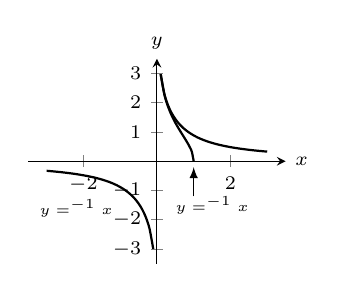
\begin{tikzpicture}
\begin{axis}[width=.4\textwidth,%
tick label style={font=\scriptsize},axis y line=middle,axis x line=middle,name=myplot,axis on top,%
			%x=.37\marginparwidth,
			%y=.37\marginparwidth,
%			xtick=\empty,% 
%			extra x ticks={.5,3},
%			extra x tick labels={$a$,$b$},
			ytick={-3,-2,-1,1,2,3},
%			yticklabels={$-0.002$,$0.002$,$0.004$},
			%minor y tick num=1,
%			extra y ticks={0.001},%
%			minor x tick num=4,
			ymin=-3.5,ymax=3.5,%
			xmin=-3.5,xmax=3.5,%
			scaled ticks=false
]



\draw (axis cs:1.5,-1.5) node {\tiny $y=\sech^{-1} x$};
\draw (axis cs:-2.2,-1.6) node {\tiny $y=\csch^{-1} x$};
\draw [->,>=latex] (axis cs:1,-1.2) -- (axis cs:1,-.2);


\addplot [{\colortwo},smooth,thick] coordinates {(-3.,-0.3275)(-2.9,-0.3383)(-2.8,-0.35)(-2.7,-0.3624)(-2.6,-0.3757)(-2.5,-0.39)(-2.4,-0.4055)(-2.3,-0.4221)(-2.2,-0.4402)(-2.1,-0.4598)(-2.,-0.4812)(-1.9,-0.5046)(-1.8,-0.5303)(-1.7,-0.5587)(-1.6,-0.5901)(-1.5,-0.6251)(-1.4,-0.6643)(-1.3,-0.7085)(-1.2,-0.7585)(-1.1,-0.8156)(-1.,-0.8814)(-0.9,-0.9578)(-0.8,-1.048)(-0.7,-1.154)(-0.6,-1.284)(-0.5,-1.444)(-0.4,-1.647)(-0.3,-1.919)(-0.2,-2.312)(-0.1,-2.998)};

\addplot [{\colortwo},smooth,thick] coordinates {(0.1,2.998)(0.2,2.312)(0.3,1.919)(0.4,1.647)(0.5,1.444)(0.6,1.284)(0.7,1.154)(0.8,1.048)(0.9,0.9578)(1.,0.8814)(1.1,0.8156)(1.2,0.7585)(1.3,0.7085)(1.4,0.6643)(1.5,0.6251)(1.6,0.5901)(1.7,0.5587)(1.8,0.5303)(1.9,0.5046)(2.,0.4812)(2.1,0.4598)(2.2,0.4402)(2.3,0.4221)(2.4,0.4055)(2.5,0.39)(2.6,0.3757)(2.7,0.3624)(2.8,0.35)(2.9,0.3383)(3.,0.3275)};

\addplot [{\colorone},thick,smooth] coordinates {(0.1,2.993)(0.2,2.292)(0.3,1.874)(0.4,1.567)(0.5,1.317)
(0.55,1.205)(0.6,1.099)(0.65,0.9961)(0.7,0.8956)(0.75,0.7954)(0.8,0.6931)(0.85,0.5857)(0.9,0.4671)(0.95,0.323)(1.,0)};
\end{axis}

\node [right] at (myplot.right of origin) {\scriptsize $x$};
\node [above] at (myplot.above origin) {\scriptsize $y$};
\end{tikzpicture}}

%\clearpage


\noindent\begin{minipage}{\textwidth}
%\centering
\small
\begin{tabular}{ccc}
Function & Domain & Range\\ \hline
$\cosh x$ & $[0,\infty)$ & $[1,\infty)$\\
$\sinh x$ & $(-\infty,\infty)$ & $(-\infty,\infty)$\\
$\tanh x$ & $(-\infty,\infty)$ & $(-1,1)$\\
$\sech x$ & $[0,\infty)$ & $(0,1]$ \\
$\csch x$ & $(-\infty,0) \cup (0,\infty)$ & $(-\infty,0) \cup (0,\infty)$\\
$\coth x$ & $(-\infty,0) \cup (0,\infty)$ & $(-\infty,-1) \cup (1,\infty)$
\end{tabular}
\hskip 40pt
%\end{minipage}\hskip 40pt
%\begin{minipage}{.7\textwidth}
%\centering\small
\begin{tabular}{ccc}
Function & Domain & Range\\ \hline
\rule{0pt}{10pt}$\cosh^{-1} x$ & $[1,\infty)$ & $[0,\infty)$ \\
$\sinh^{-1} x$ & $(-\infty,\infty)$ & $(-\infty,\infty)$\\
$\tanh^{-1} x$ & $(-1,1)$ & $(-\infty,\infty)$\\
$\sech^{-1} x$ & $(0,1]$ & $[0,\infty)$ \\
$\csch^{-1} x$ & $(-\infty,0) \cup (0,\infty)$ & $(-\infty,0) \cup (0,\infty)$\\
$\coth^{-1} x$ & $(-\infty,-1) \cup (1,\infty)$ & $(-\infty,0) \cup (0,\infty)$
\end{tabular}
%\captionsetup{type=figure}%
%\caption{Restricted domains and ranges of the hyperbolic functions.}\label{fig:hfinverse1}
\captionsetup{type=figure}%
\caption{Domains and ranges of the hyperbolic and inverse hyperbolic functions.}\label{fig:hfinverse2}
\end{minipage}
\enlargethispage{3\baselineskip}


\noindent
\begin{minipage}{\textwidth}
\begin{tabular}{ccc}
%\myincludegraphics[scale=0.95]{figures/fighfarccosh}
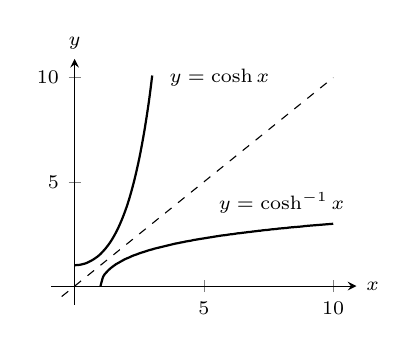
\begin{tikzpicture}
\begin{axis}[width=.45\textwidth,%
tick label style={font=\scriptsize},axis y line=middle,axis x line=middle,name=myplot,axis on top,%
			%x=.37\marginparwidth,
			%y=.37\marginparwidth,
%			xtick=\empty,% 
%			extra x ticks={.5,3},
%			extra x tick labels={$a$,$b$},
%			ytick={-.002,.002,.004},
%			yticklabels={$-0.002$,$0.002$,$0.004$},
			%minor y tick num=1,
%			extra y ticks={0.001},%
%			minor x tick num=4,
			ymin=-.9,ymax=10.9,%
			xmin=-.9,xmax=10.9,%
			scaled ticks=false
]

\addplot [{\colorone},thick,smooth] coordinates {(0,1.)(0.1,1.01) (0.2,1.02) (0.3,1.05) (0.4,1.08) (0.5,1.13) (0.6,1.19)(0.7,1.26) (0.8,1.34) (0.9,1.43) (1.,1.54) (1.1,1.67) (1.2,1.81) (1.3,1.97) (1.4,2.15) (1.5,2.35) (1.6,2.58) (1.7,2.83) (1.8,3.11)(1.9,3.42) (2.,3.76) (2.1,4.14) (2.2,4.57) (2.3,5.04) (2.4,5.56)
(2.5,6.13) (2.6,6.77) (2.7,7.47) (2.8,8.25) (2.9,9.11) (3.,10.1)};

\draw (axis cs:8,4) node {\scriptsize $y=\cosh^{-1} x$};
\draw (axis cs:5.6,10) node {\scriptsize $y=\cosh x$};

\addplot [{\colortwo},smooth,thick] coordinates {(1.,0)(1.1,0.444)(1.2,0.622)(1.3,0.756)(1.4,0.867)(1.5,0.962)(1.6,1.05)(1.7,1.12)(1.8,1.19)(1.9,1.26)(2.,1.32)(2.1,1.37)(2.2,1.43)(2.3,1.48)(2.4,1.52)(2.5,1.57)(2.6,1.61)(2.7,1.65)(2.8,1.69)(2.9,1.73)(3.,1.76)(3.1,1.8)(3.2,1.83)(3.3,1.86)(3.4,1.89)(3.5,1.92)(3.6,1.95)(3.7,1.98)(3.8,2.01)(3.9,2.04)(4.,2.06)(4.1,2.09)(4.2,2.11)(4.3,2.14)(4.4,2.16)(4.5,2.18)(4.6,2.21)(4.7,2.23)(4.8,2.25)(4.9,2.27)(5.,2.29)(5.1,2.31)(5.2,2.33)(5.3,2.35)(5.4,2.37)(5.5,2.39)(5.6,2.41)(5.7,2.43)(5.8,2.44)(5.9,2.46)(6.,2.48)(6.1,2.49)(6.2,2.51)(6.3,2.53)(6.4,2.54)(6.5,2.56)(6.6,2.57)(6.7,2.59)(6.8,2.6)(6.9,2.62)(7.,2.63)(7.1,2.65)(7.2,2.66)(7.3,2.68)(7.4,2.69)(7.5,2.7)(7.6,2.72)(7.7,2.73)(7.8,2.74)(7.9,2.76)(8.,2.77)(8.1,2.78)(8.2,2.79)(8.3,2.81)(8.4,2.82)(8.5,2.83)(8.6,2.84)(8.7,2.85)(8.8,2.86)(8.9,2.88)(9.,2.89)(9.1,2.9)(9.2,2.91)(9.3,2.92)(9.4,2.93)(9.5,2.94)(9.6,2.95)(9.7,2.96)(9.8,2.97)(9.9,2.98)(10.,2.99)};

\addplot [dashed,domain=-.5:10] {x};


%\draw (axis cs:2.4,-0.002) node {\scriptsize $f(x)$};
\end{axis}

\node [right] at (myplot.right of origin) {\scriptsize $x$};
\node [above] at (myplot.above origin) {\scriptsize $y$};
\end{tikzpicture} & \ \hskip 15pt\ &
%\myincludegraphics[scale=0.95]{figures/fighfarcsinh}
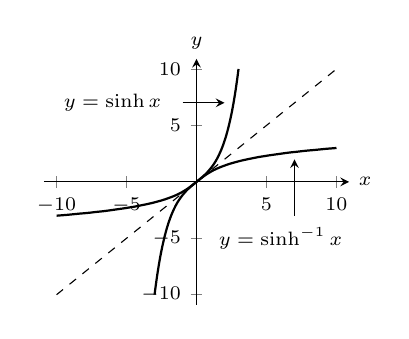
\begin{tikzpicture}
\begin{axis}[width=.45\textwidth,%
tick label style={font=\scriptsize},axis y line=middle,axis x line=middle,name=myplot,axis on top,%
			%x=.37\marginparwidth,
			%y=.37\marginparwidth,
%			xtick=\empty,% 
%			extra x ticks={.5,3},
%			extra x tick labels={$a$,$b$},
%			ytick={-.002,.002,.004},
%			yticklabels={$-0.002$,$0.002$,$0.004$},
			%minor y tick num=1,
%			extra y ticks={0.001},%
%			minor x tick num=4,
			ymin=-10.9,ymax=10.9,%
			xmin=-10.9,xmax=10.9,%
			scaled ticks=false
]

\addplot [{\colorone},thick,smooth] coordinates {(-3.,-10.) (-2.9,-9.06) (-2.8,-8.19) (-2.7,-7.41) (-2.6,-6.69)(-2.5,-6.05) (-2.4,-5.47) (-2.3,-4.94) (-2.2,-4.46) (-2.1,-4.02)(-2.,-3.63) (-1.9,-3.27) (-1.8,-2.94) (-1.7,-2.65) (-1.6,-2.38)(-1.5,-2.13) (-1.4,-1.9) (-1.3,-1.7) (-1.2,-1.51) (-1.1,-1.34)(-1.,-1.18) (-0.9,-1.03) (-0.8,-0.888) (-0.7,-0.759) (-0.6,-0.637)(-0.5,-0.521) (-0.4,-0.411) (-0.3,-0.305) (-0.2,-0.201) (-0.1,-0.1)(0,0) (0.1,0.1) (0.2,0.201) (0.3,0.305) (0.4,0.411) (0.5,0.521)(0.6,0.637) (0.7,0.759) (0.8,0.888) (0.9,1.03) (1.,1.18) (1.1,1.34)(1.2,1.51) (1.3,1.7) (1.4,1.9) (1.5,2.13) (1.6,2.38) (1.7,2.65)(1.8,2.94) (1.9,3.27) (2.,3.63) (2.1,4.02) (2.2,4.46) (2.3,4.94)(2.4,5.47) (2.5,6.05) (2.6,6.69) (2.7,7.41) (2.8,8.19) (2.9,9.06)(3.,10.) };

\draw (axis cs:-6,7) node {\scriptsize $y=\sinh x$};
\draw (axis cs:6,-5) node {\scriptsize $y=\sinh^{-1} x$};
\draw[->,>=stealth] (axis cs:-1,7) -- (axis cs:2,7);
\draw[->,>=stealth] (axis cs:7,-3) -- (axis cs:7,2);

\addplot [{\colortwo},smooth,thick] coordinates {(-10.,-3.)(-9.6,-2.96)(-9.2,-2.92)(-8.8,-2.87)(-8.4,-2.82)(-8.,-2.78)(-7.6,-2.73)(-7.2,-2.67)(-6.8,-2.62)(-6.4,-2.56)(-6.,-2.49)(-5.6,-2.42)(-5.2,-2.35)(-4.8,-2.27)(-4.4,-2.19)(-4.,-2.09)(-3.6,-1.99)(-3.2,-1.88)(-2.8,-1.75)(-2.4,-1.61)(-2.,-1.44)(-1.6,-1.25)(-1.2,-1.02)(-0.8,-0.733)(-0.4,-0.39)(0,0)(0.4,0.39)(0.8,0.733)(1.2,1.02)(1.6,1.25)(2.,1.44)(2.4,1.61)(2.8,1.75)(3.2,1.88)(3.6,1.99)(4.,2.09)(4.4,2.19)(4.8,2.27)(5.2,2.35)(5.6,2.42)(6.,2.49)(6.4,2.56)(6.8,2.62)(7.2,2.67)(7.6,2.73)(8.,2.78)(8.4,2.82)(8.8,2.87)(9.2,2.92)(9.6,2.96)(10.,3.)};

\addplot [dashed,domain=-10:10] {x};


%\draw (axis cs:2.4,-0.002) node {\scriptsize $f(x)$};
\end{axis}

\node [right] at (myplot.right of origin) {\scriptsize $x$};
\node [above] at (myplot.above origin) {\scriptsize $y$};
\end{tikzpicture}\\[15pt]
%\myincludegraphics[scale=0.95]{figures/fighfarctanharccoth} 
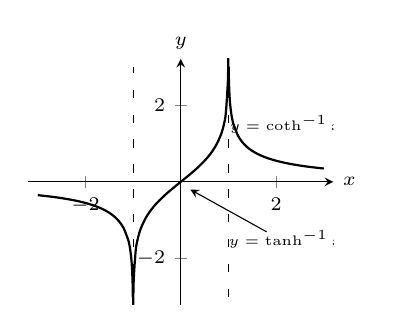
\begin{tikzpicture}
\begin{axis}[width=.45\textwidth,%
tick label style={font=\scriptsize},axis y line=middle,axis x line=middle,name=myplot,axis on top,%
			%x=.37\marginparwidth,
			%y=.37\marginparwidth,
			xtick={-2,2},%
%			xticklabels={$-1\qquad $,$\quad 1$}, 
%			extra x ticks={.5,3},
%			extra x tick labels={$a$,$b$},
			ytick={-2,2},
%			yticklabels={$-0.002$,$0.002$,$0.004$},
			%minor y tick num=1,
%			extra y ticks={0.001},%
%			minor x tick num=4,
			ymin=-3.2,ymax=3.2,%
			xmin=-3.2,xmax=3.2,%
			scaled ticks=false
]

%\addplot [{\colorone},thick,smooth] coordinates {(-3.,-0.995)(-2.9,-0.994)(-2.8,-0.993)(-2.7,-0.991)(-2.6,-0.989)(-2.5,-0.987)(-2.4,-0.984)(-2.3,-0.98)(-2.2,-0.976)(-2.1,-0.97)(-2.,-0.964)(-1.9,-0.956)(-1.8,-0.947)(-1.7,-0.935)(-1.6,-0.922)(-1.5,-0.905)(-1.4,-0.885)(-1.3,-0.862)(-1.2,-0.834)(-1.1,-0.8)(-1.,-0.762)(-0.9,-0.716)(-0.8,-0.664)(-0.7,-0.604)(-0.6,-0.537)(-0.5,-0.462)(-0.4,-0.38)(-0.3,-0.291)(-0.2,-0.197)(-0.1,-0.0997)(0,0)(0.1,0.0997)(0.2,0.197)(0.3,0.291)(0.4,0.38)(0.5,0.462)(0.6,0.537)(0.7,0.604)(0.8,0.664)(0.9,0.716)(1.,0.762)(1.1,0.8)(1.2,0.834)(1.3,0.862)(1.4,0.885)(1.5,0.905)(1.6,0.922)(1.7,0.935)(1.8,0.947)(1.9,0.956)(2.,0.964)(2.1,0.97)(2.2,0.976)(2.3,0.98)(2.4,0.984)(2.5,0.987)(2.6,0.989)(2.7,0.991)(2.8,0.993)(2.9,0.994)(3.,0.995)};

\addplot [{\colortwo},thick,smooth] coordinates {(1.005,2.997)(1.01,2.65)(1.02,2.31)(1.03,2.11)(1.04,1.97)(1.05,1.86)(1.06,1.77)(1.07,1.69)(1.08,1.63)(1.09,1.57)(1.1,1.52)(1.2,1.2)(1.3,1.02)(1.4,0.896)(1.5,0.805)(1.6,0.733)(1.7,0.675)(1.8,0.626)(1.9,0.585)(2.,0.549)(2.1,0.518)(2.2,0.49)(2.3,0.466)(2.4,0.444)(2.5,0.424)(2.6,0.405)(2.7,0.389)(2.8,0.374)(2.9,0.36)(3.,0.347)};

\addplot [{\colortwo},thick,smooth] coordinates {(-3.,-0.347)(-2.9,-0.36)(-2.8,-0.374)(-2.7,-0.389)(-2.6,-0.405)(-2.5,-0.424)(-2.4,-0.444)(-2.3,-0.466)(-2.2,-0.49)(-2.1,-0.518)(-2.,-0.549)(-1.9,-0.585)(-1.8,-0.626)(-1.7,-0.675)(-1.6,-0.733)(-1.5,-0.805)(-1.4,-0.896)(-1.3,-1.02)(-1.2,-1.2)(-1.1,-1.52)(-1.09,-1.57)(-1.08,-1.63)(-1.07,-1.69)(-1.06,-1.77)(-1.05,-1.86)(-1.04,-1.97)(-1.03,-2.11)(-1.02,-2.31)(-1.01,-2.65)(-1.005,-2.997)};

\draw (axis cs:2.2,1.5) node {\tiny $y=\coth^{-1} x$};
\draw (axis cs:2.2,-1.5) node {\tiny $y=\tanh^{-1} x$};
\draw [->,>=stealth] (axis cs:1.8,-1.3) -- (axis cs:.2,-.2);
%\draw [->,>=stealth] (axis cs:-.1,2.5) -- (axis cs:.7,2.5);
\draw [loosely dashed] (axis cs:-1,-3)--(axis cs:-1,3);
\draw [loosely dashed] (axis cs:1,-3)--(axis cs:1,3);


\addplot [{\colorone},smooth,thick] coordinates {(-0.999,-3.8)(-0.99,-2.65)(-0.945,-1.78)(-0.9,-1.47)(-0.855,-1.27)(-0.81,-1.13)(-0.765,-1.01)(-0.72,-0.908)(-0.675,-0.82)(-0.63,-0.741)(-0.585,-0.67)(-0.54,-0.604)(-0.495,-0.543)(-0.45,-0.485)(-0.405,-0.43)(-0.36,-0.377)(-0.315,-0.326)(-0.27,-0.277)(-0.225,-0.229)(-0.18,-0.182)(-0.135,-0.136)(-0.09,-0.0902)(-0.045,-0.045)(0,0)(0.045,0.045)(0.09,0.0902)(0.135,0.136)(0.18,0.182)(0.225,0.229)(0.27,0.277)(0.315,0.326)(0.36,0.377)(0.405,0.43)(0.45,0.485)(0.495,0.543)(0.54,0.604)(0.585,0.67)(0.63,0.741)(0.675,0.82)(0.72,0.908)(0.765,1.01)(0.81,1.13)(0.855,1.27)(0.9,1.47)(0.945,1.78)(0.99,2.65)(0.994,2.95)(0.999,3.8)};

\end{axis}

\node [right] at (myplot.right of origin) {\scriptsize $x$};
\node [above] at (myplot.above origin) {\scriptsize $y$};
\end{tikzpicture}
& & %\myincludegraphics[scale=0.95]{figures/fighfarcsecharccsch}
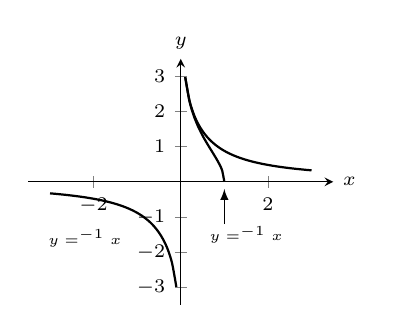
\begin{tikzpicture}
\begin{axis}[width=.45\textwidth,%
tick label style={font=\scriptsize},axis y line=middle,axis x line=middle,name=myplot,axis on top,%
			%x=.37\marginparwidth,
			%y=.37\marginparwidth,
%			xtick=\empty,% 
%			extra x ticks={.5,3},
%			extra x tick labels={$a$,$b$},
			ytick={-3,-2,-1,1,2,3},
%			yticklabels={$-0.002$,$0.002$,$0.004$},
			%minor y tick num=1,
%			extra y ticks={0.001},%
%			minor x tick num=4,
			ymin=-3.5,ymax=3.5,%
			xmin=-3.5,xmax=3.5,%
			scaled ticks=false
]



\draw (axis cs:1.5,-1.5) node {\tiny $y=\sech^{-1} x$};
\draw (axis cs:-2.2,-1.6) node {\tiny $y=\csch^{-1} x$};
\draw [->,>=latex] (axis cs:1,-1.2) -- (axis cs:1,-.2);


\addplot [{\colortwo},smooth,thick] coordinates {(-3.,-0.3275)(-2.9,-0.3383)(-2.8,-0.35)(-2.7,-0.3624)(-2.6,-0.3757)(-2.5,-0.39)(-2.4,-0.4055)(-2.3,-0.4221)(-2.2,-0.4402)(-2.1,-0.4598)(-2.,-0.4812)(-1.9,-0.5046)(-1.8,-0.5303)(-1.7,-0.5587)(-1.6,-0.5901)(-1.5,-0.6251)(-1.4,-0.6643)(-1.3,-0.7085)(-1.2,-0.7585)(-1.1,-0.8156)(-1.,-0.8814)(-0.9,-0.9578)(-0.8,-1.048)(-0.7,-1.154)(-0.6,-1.284)(-0.5,-1.444)(-0.4,-1.647)(-0.3,-1.919)(-0.2,-2.312)(-0.1,-2.998)};

\addplot [{\colortwo},smooth,thick] coordinates {(0.1,2.998)(0.2,2.312)(0.3,1.919)(0.4,1.647)(0.5,1.444)(0.6,1.284)(0.7,1.154)(0.8,1.048)(0.9,0.9578)(1.,0.8814)(1.1,0.8156)(1.2,0.7585)(1.3,0.7085)(1.4,0.6643)(1.5,0.6251)(1.6,0.5901)(1.7,0.5587)(1.8,0.5303)(1.9,0.5046)(2.,0.4812)(2.1,0.4598)(2.2,0.4402)(2.3,0.4221)(2.4,0.4055)(2.5,0.39)(2.6,0.3757)(2.7,0.3624)(2.8,0.35)(2.9,0.3383)(3.,0.3275)};

\addplot [{\colorone},thick,smooth] coordinates {(0.1,2.993)(0.2,2.292)(0.3,1.874)(0.4,1.567)(0.5,1.317)
(0.55,1.205)(0.6,1.099)(0.65,0.9961)(0.7,0.8956)(0.75,0.7954)(0.8,0.6931)(0.85,0.5857)(0.9,0.4671)(0.95,0.323)(1.,0)};
\end{axis}

\node [right] at (myplot.right of origin) {\scriptsize $x$};
\node [above] at (myplot.above origin) {\scriptsize $y$};
\end{tikzpicture}
\end{tabular}
\captionsetup{type=figure}%
\caption{Graphs of the hyperbolic functions and their inverses.}\label{fig:hfinverse1}
\end{minipage}



\begin{definition}{Logarithmic definitions of Inverse Hyperbolic Functions}{idea:hyperbolic_log}
{\noindent%
\begin{minipage}[t]{.55\textwidth}
\begin{enumerate}
\item $\ds\cosh^{-1}x=\ln\big(x+\sqrt{x^2-1}\big);\ x\geq1$\index{hyperbolic function!inverse!logarithmic def.}\rule[-10pt]{0pt}{20pt}
\item $\ds\tanh^{-1}x = \frac12\ln\left(\frac{1+x}{1-x}\right);\ |x|<1$\rule[-10pt]{0pt}{20pt}
\item $\ds \sech^{-1}x = \ln\left(\frac{1+\sqrt{1-x^2}}x\right);\ 0<x\leq1$\rule[-10pt]{0pt}{20pt}
\end{enumerate}
\end{minipage}
\begin{minipage}[t]{.5\textwidth}
\begin{enumerate}\addtocounter{enumi}{3}
\item $\ds\sinh^{-1}x = \ln\big(x+\sqrt{x^2+1}\big)$\rule[-10pt]{0pt}{20pt}
\item	 $\ds\coth^{-1}x = \frac12\ln\left(\frac{x+1}{x-1}\right);\ |x|>1$\rule[-10pt]{0pt}{20pt}
\item $\ds\csch^{-1}x = \ln\left(\frac1x+\frac{\sqrt{1+x^2}}{|x|}\right);\ x\neq0$\rule[-10pt]{0pt}{20pt}
\end{enumerate}
\end{minipage}
}
\end{definition}



The following gives the derivatives and integrals relating to the inverse hyperbolic functions. Both the inverse hyperbolic and logarithmic function representations of the antiderivative are given, based on Definition \ref{def:idea:hyperbolic_log}. Again, these latter functions are often more useful than the former. Note how inverse hyperbolic functions can be used to solve integrals we used Trigonometric Substitution to solve in Section \ref{sec:trig_sub}.



%\mtable{.62}{Logarithmic definitions of the inverse hyperbolic functions.}{fig:hfinverse5}{%
%\begin{align*}
%\cosh^{-1}x&=\ln\big(x+\sqrt{x^2-1}\big);\ x\geq1\\
%\sinh^{-1}x &= \ln\big(x+\sqrt{x^2+1}\big)\\
%\tanh^{-1}x &= \frac12\ln\left(\frac{1+x}{1-x}\right);\ |x|<1\\
%\sech^{-1}x &= \ln\left(\frac{1+\sqrt{1-x^2}}x\right);\ 0<x\leq1\\
%\csch^{-1}x &= \ln\left(\frac1x+\frac{\sqrt{1+x^2}}{|x|}\right);\ x\neq0\\
%\coth^{-1}x &= \frac12\ln\left(\frac{x+1}{x-1}\right);\ |x|>1
%\end{align*}
%}


\begin{formulabox}[{Derivatives Involving Inverse Hyperbolic Functions}]
\label{idea:hyperbolic_inverse_derivatives}
{%
\begin{minipage}[t]{.45\textwidth}
\begin{enumerate}
\item $\ds\frac{d}{dx}\big(\cosh^{-1} x\big) = \frac{1}{\sqrt{x^2-1}};\ x>1$\index{derivative!inverse hyper.}\index{hyperbolic function!inverse!derivative}
\item $\ds\frac{d}{dx}\big(\sinh^{-1} x\big) = \frac{1}{\sqrt{x^2+1}}$
\item $\ds\frac{d}{dx}\big(\tanh^{-1} x\big) = \frac{1}{1-x^2};\ |x|<1$
\end{enumerate}
\end{minipage}
\begin{minipage}[t]{.55\textwidth}
\begin{enumerate}\addtocounter{enumi}{3}
\item $\ds\frac{d}{dx}\big(\sech^{-1} x\big) = \frac{-1}{x\sqrt{1-x^2}}; 0<x<1$
\item $\ds\frac{d}{dx}\big(\csch^{-1} x\big) = \frac{-1}{|x|\sqrt{1+x^2}};\ x\neq0$
\item $\ds\frac{d}{dx}\big(\coth^{-1} x\big) = \frac{1}{1-x^2};\ |x|>1$
\end{enumerate}
\end{minipage}
}
\end{formulabox}


\begin{formulabox}[{Integrals Involving Inverse Hyperbolic Functions}]
\label{idea:hyperbolic_inverse_integrals}
{%
\begin{enumerate}
\item \parbox{70pt}{$\ds\int \frac{1}{\sqrt{x^2-a^2}}\ dx$} \parbox{180pt}{$\ds=\qquad \cosh^{-1}\left(\frac xa\right)+C;\ 0<a<x$} $\ds=\ln\Big|x+\sqrt{x^2-a^2}\Big|+C$\index{integration!inverse hyper.}\index{hyperbolic function!inverse!integration}

\item \parbox{70pt}{$\ds\int \frac{1}{\sqrt{x^2+a^2}}\ dx$} \parbox{180pt}{$\ds=\qquad \sinh^{-1}\left(\frac xa\right)+C;\ a>0$} $\ds=\ln\Big|x+\sqrt{x^2+a^2}\Big|+C$

\item \parbox{70pt}{$\ds\int \frac{1}{a^2-x^2}\ dx$} \parbox{180pt}{$\ds=\qquad \left\{\begin{array}{ccc} \frac1a\tanh^{-1}\left(\frac xa\right)+C & & x^2<a^2 \\ \\
\frac1a\coth^{-1}\left(\frac xa\right)+C & & a^2<x^2 \end{array}\right.$} $\ds=\frac12\ln\left|\frac{a+x}{a-x}\right|+C$

\item \parbox{70pt}{$\ds\int \frac{1}{x\sqrt{a^2-x^2}}\ dx $} \parbox{180pt}{$\ds=\qquad -\frac1a\sech^{-1}\left(\frac xa\right)+C;\ 0<x<a$} $\ds= \frac1a \ln\left(\frac{x}{a+\sqrt{a^2-x^2}}\right)+C $

\item	\parbox{70pt}{$\ds\int \frac{1}{x\sqrt{x^2+a^2}}\ dx $} \parbox{180pt}{$\ds=\qquad -\frac1a\csch^{-1}\left|\frac xa\right| + C;\ x\neq 0,\ a>0$}$\ds= \frac1a \ln\left|\frac{x}{a+\sqrt{a^2+x^2}}\right|+C $
\end{enumerate}
%\end{minipage}
}
\end{formulabox}

We practice using the derivative and integral formulas in the following example.\\


\begin{example}{Derivatives and integrals involving inverse hyperbolic functions}{ex_hf3}
{Evaluate the following.

\noindent%
\begin{minipage}[t]{.5\textwidth}
\begin{enumerate}
\item	$\ds \frac{d}{dx}\left[\cosh^{-1}\left(\frac{3x-2}{5}\right)\right]$
\item	$\ds \int\frac{1}{x^2-1}\ dx$
\end{enumerate}
\end{minipage}
\begin{minipage}[t]{.5\textwidth}
\begin{enumerate}\addtocounter{enumi}{2}
\item	$\ds \int \frac{1}{\sqrt{9x^2+10}}\ dx$
\end{enumerate}
\end{minipage}
}
\end{example}


\begin{solution}
{\begin{enumerate}
\item	Applying the Chain Rule gives:
		$$\frac{d}{dx}\left[\cosh^{-1}\left(\frac{3x-2}5\right)\right] = \frac{1}{\sqrt{\left(\frac{3x-2}5\right)^2-1}}\cdot\frac35.$$

\item		Multiplying the numerator and denominator by $(-1)$ gives: $\ds \int \frac{1}{x^2-1}\ dx = \int \frac{-1}{1-x^2}\ dx$. The second integral can be solved with a direct application of item \#3 from Integrals Involving Inverse Hyperbolic Functions, with $a=1$. Thus
\begin{align}
\int \frac{1}{x^2-1}\ dx &= -\int \frac{1}{1-x^2}\ dx \notag \\
		&= \left\{\begin{array}{ccc} -\tanh^{-1}\left(x\right)+C & & x^2<1 \\ \\
-\coth^{-1}\left(x\right)+C & & 1<x^2 \end{array}\right. \notag\\
     &=-\frac12\ln\left|\frac{x+1}{x-1}\right|+C\notag\\
     &=\frac12\ln\left|\frac{x-1}{x+1}\right|+C.\label{eq:hf3}
     \end{align}

We should note that this exact problem was solved at the beginning of Section \ref{sec:partial_fraction}. In that example the answer was given as $\frac12\ln|x-1|-\frac12\ln|x+1|+C.$ Note that this is equivalent to the answer given in Equation \ref{eq:hf3}, as $\ln(a/b) = \ln a - \ln b$.

%The key to linking the two seemingly different answers together is Figure \ref{fig:hfinverse5}, where the logarithmic definitions of the inverse hyperbolic functions are given. Note that the definitions of $\tanh^{-1}x$ and $\coth^{-1}x$ are very similar; the conditions placed on $|x|$ ensure that the argument of $\ln$ is always positive. Thus one could say 
%$$\frac12\ln\left|\frac{x+1}{x-1}\right| = \left\{\begin{array}{ccc} \tanh^{-1}x+C & & |x|<1 \\ \\
%\coth^{-1}x+C & & |x|>1 \end{array}\right..$$
%
%We reconcile the two answers by returning to Equation \ref{eq:hf3} and continuing:
%\begin{align*}
%\int \frac{1}{x^2-1}\ dx &= \int \frac{-1}{1-x^2}\ dx \\
%			&= \left\{\begin{array}{ccc} -\frac1a\tanh^{-1}\left(\frac xa\right)+C & & x^2<a^2 \\ \\
%-\frac1a\coth^{-1}\left(\frac xa\right)+C & & a^2<x^2 \end{array}\right. \\
%			&= -\frac12\ln\left|\frac{x+1}{x-1}\right|+C \\
%			&= -\frac12\ln|x+1| + \frac12\ln|x-1| +C,
%\end{align*}
%matching the answer previously obtained.

\item		This requires a substitution, then item \#2 of Integrals Involving Inverse Hyperbolic Functions can be applied.

Let $u = 3x$, hence $du = 3dx$. We have 
\begin{align*}
\int \frac{1}{\sqrt{9x^2+10}}\ dx &= \frac13\int\frac{1}{\sqrt{u^2+10}}\ du. \\
		\intertext{Note $a^2=10$, hence $a = \sqrt{10}.$ Now apply the integral rule.}\\
		 &= \frac13 \sinh^{-1}\left(\frac{3x}{\sqrt{10}}\right) + C \\
		 &= \frac13 \ln \Big|3x+\sqrt{9x^2+10}\Big|+C.
\end{align*}
\end{enumerate}
\vskip-\baselineskip
}
\end{solution}





This section covers a lot of ground. New functions were introduced, along with some of their fundamental identities, their derivatives and antiderivatives, their inverses, and the derivatives and antiderivatives of these inverses. 
%Four Key Ideas were presented, each including quite a bit of information.

Do not view this section as containing a source of information to be memorized, but rather as a reference for future problem solving. 

%Key Idea \ref{idea:hyperbolic_inverse_integrals} contains perhaps the most useful information. Know the integration forms it helps evaluate and understand how to use the inverse hyperbolic answer and the logarithmic answer.
%
%The next section takes a brief break from demonstrating new integration techniques. It instead demonstrates a technique of evaluating limits that return indeterminate forms. This technique will be useful in Section \ref{sec:improper_integration}, where limits will arise in the evaluation of certain definite integrals.

%%%%%%%%%%%%%%%%%%%%%%%%%%%%%%%%%%%%%%%%%%%%%%%%%
\Opensolutionfile{solutions}[ex]
\section*{Exercises for Section \ref{sec:hyperbolic revisited}}

\begin{enumialphparenastyle}


\begin{ex}
Verify the given identity.
\begin{enumerate}
\item {$\ds\frac{d}{dx}\left[\sech x\right] = -\sech x\tanh x$}

\item {$\ds\frac{d}{dx}\left[\coth x\right] = -\csch^2x$}
\item {$\ds \int \tanh x\ dx  = \ln (\cosh x) + C$}

\item {$\ds \int \coth x\ dx  = \ln |\sinh x| + C$}

\end{enumerate}
	\begin{sol}
		\begin{enumerate}
		\item {\hfill$\begin{aligned}[t]
				\frac{d}{dx}\left[\sech x\right] &= \frac{d}{dx}\left[\frac{2}{e^x+e^{-x}}\right]  \\
													&= \frac{-2(e^x-e^{-x})}{(e^x+e^{-x})^2} \\
													&= -\frac{2(e^x-e^{-x})}{(e^x+e^{-x})(e^x+e^{-x})} \\
													&= -\frac{2}{e^x+e^{-x}}\cdot \frac{e^x-e^{-x}}{e^x+e^{-x}}\\
													&= -\sech x\tanh x
		\end{aligned}$\hfill\null}
		\item 
		{\hfill$\begin{aligned}[t]
				\frac{d}{dx}\left[\coth x\right] &= \frac{d}{dx}\left[\frac{e^x+e^{-x}}{e^x-e^{-x}}\right]  \\
													&= \frac{(e^x-e^{-x})(e^x-e^{-x})-(e^x+e^{-x})(e^x+e^{-x})}{(e^x-e^{-x})^2}\\
													&= \frac{e^{2x}+e^{-2x} - 2 - (e^{2x}+e^{-2x}+2)}{(e^x-e^{-x})^2}\\
													&= -\frac{4}{(e^x-e^{-x})^2}\\
													&=-\csch^2x
		\end{aligned}$\hfill\null}
		\item {$\ds	\int \tanh x\ dx = \int \frac{\sinh x}{\cosh x}\ dx$\\
		Let $u = \cosh x$; $du = (\sinh x) dx$\\
		\hfill$\begin{aligned}[t]
													&= \int \frac{1}{u}\ du \\
													&= \ln |u| + C \\
													&= \ln (\cosh x) + C.
		\end{aligned}$\hfill\null}
		\item {\hfill$\begin{aligned}[t]
				\int \coth x\ dx &= \int \frac{\cosh x}{\sinh x}\ dx\\
													\text{Let $u = \sinh x$; $du = (\cosh x) dx$} 	\\
													&= \int \frac{1}{u}\ du \\
													&= \ln |u| + C \\
													&= \ln |\sinh x| + C.
		\end{aligned}$\hfill\null}
		\end{enumerate}
	\end{sol}
\end{ex}

\begin{ex}
Find the derivative of the given function.
\begin{enumerate}
\item {$f(x) = \cosh 2x$}

\item {$f(x) = \tanh (x^2)$}

\item {$f(x) = \ln(\sinh x)$}

\item {$f(x) = \sinh x\cosh x$}

\item {$f(x) = x\sinh x-\cosh x$}

\item {$f(x) = \sech^{-1} (x^2)$}

\item {$f(x) = \sinh^{-1} (3x)$}

\item {$f(x) = \cosh^{-1} (2x^2)$}

\item {$f(x) = \tanh^{-1} (x+5)$}

\item {$f(x) = \tanh^{-1} (\cos x)$}

\item {$f(x) = \cosh^{-1} (\sec x)$}

\end{enumerate}
	\begin{sol}
	\begin{enumerate}
	\item {$2\sinh 2x$}
	\item {$2x\sec^2(x^2)$}
	\item {$\coth x$}
	\item {$\sinh^2x+\cosh^2x$}
	\item {$x\cosh x$}
	\item {$\frac{-2x}{(x^2)\sqrt{1-x^4}}$}
	\item {$\frac{3}{\sqrt{9x^2+1}}$}
	\item {$\frac{4x}{\sqrt{4x^4-1}}$}
	\item {$\frac{1}{1-(x+5)^2}$}
	\item {$-\csc x$}
	\item {$\sec x$}
	\end{enumerate}
	\end{sol}
\end{ex}


\begin{ex}
Find the equation of the line tangent to the function at the given $x$-value.
\begin{enumerate}
\item {$f(x) = \sinh x$ at $x=0$}

\item {$f(x) = \cosh x$ at $x=\ln 2$}

\item {$f(x) = \sech^2 x$ at $x=\ln 3$}

\item {$f(x) = \sinh^{-1} x$ at $x=0$}

\item {$f(x) = \cosh^{-1} x$ at $x=\sqrt 2$}

\end{enumerate}
	\begin{sol}
	\begin{enumerate}
	\item {$y=x$}
	\item {$y=3/4(x-\ln 2)+5/4$}
	\item {$y=-72/125(x-\ln 3)+9/25$}
	\item {$y=x$}
	\item  {$y=(x-\sqrt{2})+\cosh^{-1}(\sqrt{2}) \approx (x-1.414)+0.881$}
	\end{enumerate}
	\end{sol}
\end{ex}


\begin{ex}
Evaluate the given indefinite integral.
\begin{enumerate}
\item {$\ds \int \tanh (2x)\ dx$}

\item {$\ds \int \cosh (3x-7)\ dx$}

\item {$\ds \int \sinh x\cosh x\ dx$}

\item {$\ds \int x\cosh x\ dx$}

\item {$\ds \int x\sinh x\ dx$}

\item {$\ds \int \frac{1}{9-x^2}\ dx$}

\item {$\ds \int \frac{2x}{\sqrt{x^4-4}}\ dx$}

\item {$\ds \int \frac{\sqrt{x}}{\sqrt{1+x^3}}\ dx$}

\item {$\ds \int \frac{1}{x^4-16}\ dx$}

\item {$\ds \int \frac{1}{x^2+x}\ dx$}

\item {$\ds \int \frac{e^x}{e^{2x}+1}\ dx$}

\item {$\ds \int \sinh^{-1}x \ dx$}

\item {$\ds \int \tanh^{-1}x \ dx$}

\item {$\ds \int \sech x \ dx$ \quad(Hint: mutiply by $\frac{\cosh x}{\cosh x}$; set $u = \sinh x$.)}

\end{enumerate}
	\begin{sol}
	\begin{enumerate}
	\item {$1/2\ln (\cosh(2x))+C$}
	\item {$1/3\sinh(3x-7)+C$}
	\item {$1/2\sinh^2x+C$ or $1/2\cosh^2x+C$}
	\item {$x \sinh (x)-\cosh (x)+C$
	}
	\item {$x \cosh (x)-\sinh (x)+C$
	}
	\item {$\left\{\begin{array}{ccc} \frac13\tanh^{-1}\left(\frac x3\right)+C & & x^2<9 \\ \\
	\frac13\coth^{-1}\left(\frac x3\right)+C & & 9<x^2 \end{array}\right. = \frac12\ln |x+1| - \frac12\ln |x-1|+C$} 
	\item  {$\cosh^{-1} (x^2/2) + C = \ln (x^2+\sqrt{x^4-4})+C$}
	\item {$2/3\sinh^{-1} x^{3/2} + C = 2/3\ln (x^{3/2}+\sqrt{x^3+1})+C$}
	\item {$\frac{1}{16}\tan^{-1}(x/2)+\frac{1}{32}\ln |x-2|+\frac1{32}\ln|x+2|+C$}
	\item {$\ln x- \ln|x+1|+C$}
	\item {$\tan^{-1}(e^x)+C$}
	\item {$x\sinh^{-1}x-\sqrt{x^2+1}+C$}
	\item {$x\tanh^{-1}x+1/2\ln|x^2-1|+C$}
	\item  {$\tan^{-1}(\sinh x)+C$} 
	\end{enumerate}
	\end{sol}
\end{ex}


\begin{ex}
Evaluate the given definite integral.
\begin{enumerate}
\item {$\ds \int_{-1}^1 \sinh x \ dx$}

\item {$\ds \int_{-\ln 2}^{\ln 2} \cosh x \ dx$}
\item {$\ds \int_{0}^{1} \tanh^{-1} x \ dx$}
\end{enumerate}
	\begin{sol}
	\begin{enumerate}
	\item {$0$}
	\item {$3/2$}
	
	\item {$2$}  
	\end{enumerate}
	\end{sol}
\end{ex}





\end{enumialphparenastyle}
